\documentclass[a4paper,11pt]{article}
\usepackage{amsmath}
\usepackage[english]{babel}
\usepackage{color}
\usepackage{graphicx}
\usepackage{hyperref}
\usepackage{mathabx}

\DeclareMathOperator*{\argmax}{arg\,max}
\DeclareMathOperator*{\chol}{cholesky}
\DeclareMathOperator*{\err}{E}
\newcommand{\V}[1]{\ensuremath{\boldsymbol{#1}}}
\newcommand{\T}[1]{\ensuremath{\mathtt{#1}}}
\newcommand{\mean}{\ensuremath{\boldsymbol{\mu}}}
\newcommand{\cov}{\ensuremath{\boldsymbol{\Sigma}}}
\newcommand{\npdf}{\ensuremath{\mathcal{N}}}
\newcommand{\dif}{\ensuremath{\mathrm{d}}}

\newcommand{\hl}[1]{\colorbox{cyan}{#1}}
\newcommand{\mhl}[1]{\mathchoice%
  {\colorbox{cyan}{$\displaystyle#1$}}%
  {\colorbox{cyan}{$\textstyle#1$}}%
  {\colorbox{cyan}{$\scriptstyle#1$}}%
  {\colorbox{cyan}{$\scriptscriptstyle#1$}}}

\title{Lab 4: Gaussian Processes}
\author{Patrick de Kok}
\begin{document}
\maketitle

In this exercise, I have learnt how to use Gaussian processes on sparse data, such as the \texttt{chirps.mat} dataset.  The data has been split in a train set of 12 data points and a test set of 3 data points.  The data points have been randomly divided into either set.


\section{The Gaussian distribution}
\begin{figure}
  \begin{center}
    \caption[Plot of the Gaussian distribution with covariance $\cov_{1,1} = 1, \cov_{2,2} = 3$.]{Plot of the Gaussian distribution with mean $\mean = 0$ and covariance $\cov = \begin{bmatrix}1 & 0\\0 & 3\end{bmatrix}$.  In the plot above, one can see the contour plot of $\mathcal G_1 = \npdf(\V{x} ; \mean, \cov)$ with isolines for points with probability density $0.01, 0.02, \ldots 0.09$.  The lower plot shows the marginal distribution over $x_1$.}
    \label{fig:plot1}
    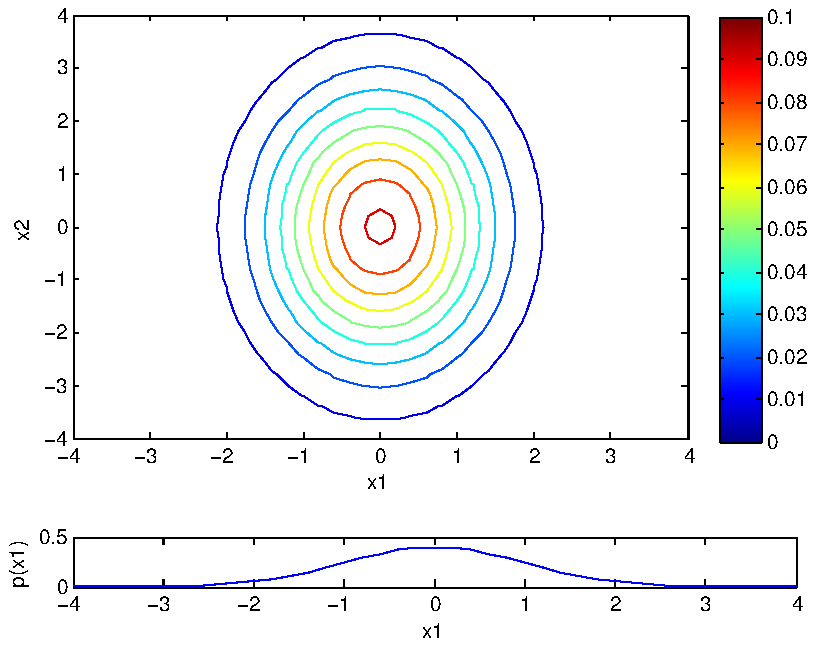
\includegraphics[width=0.8\textwidth]{ex1plot1}
  \end{center}
\end{figure}
\begin{figure}
  \begin{center}
    \caption{Plots of the conditional distribution over $x_1$ given various values for $x_2$ given the Gaussian distribution $\mathcal G_1$.  The conditional distribution over $x_1$ is plotted from top to bottom for $x_2 = -3$, $x_2 = -2$, $x_2 = -1$, $x_2 = 0$, $x_2 = 1$, $x_2 = 2$ and $x_2 = 3$.}
    \label{fig:plot2}
    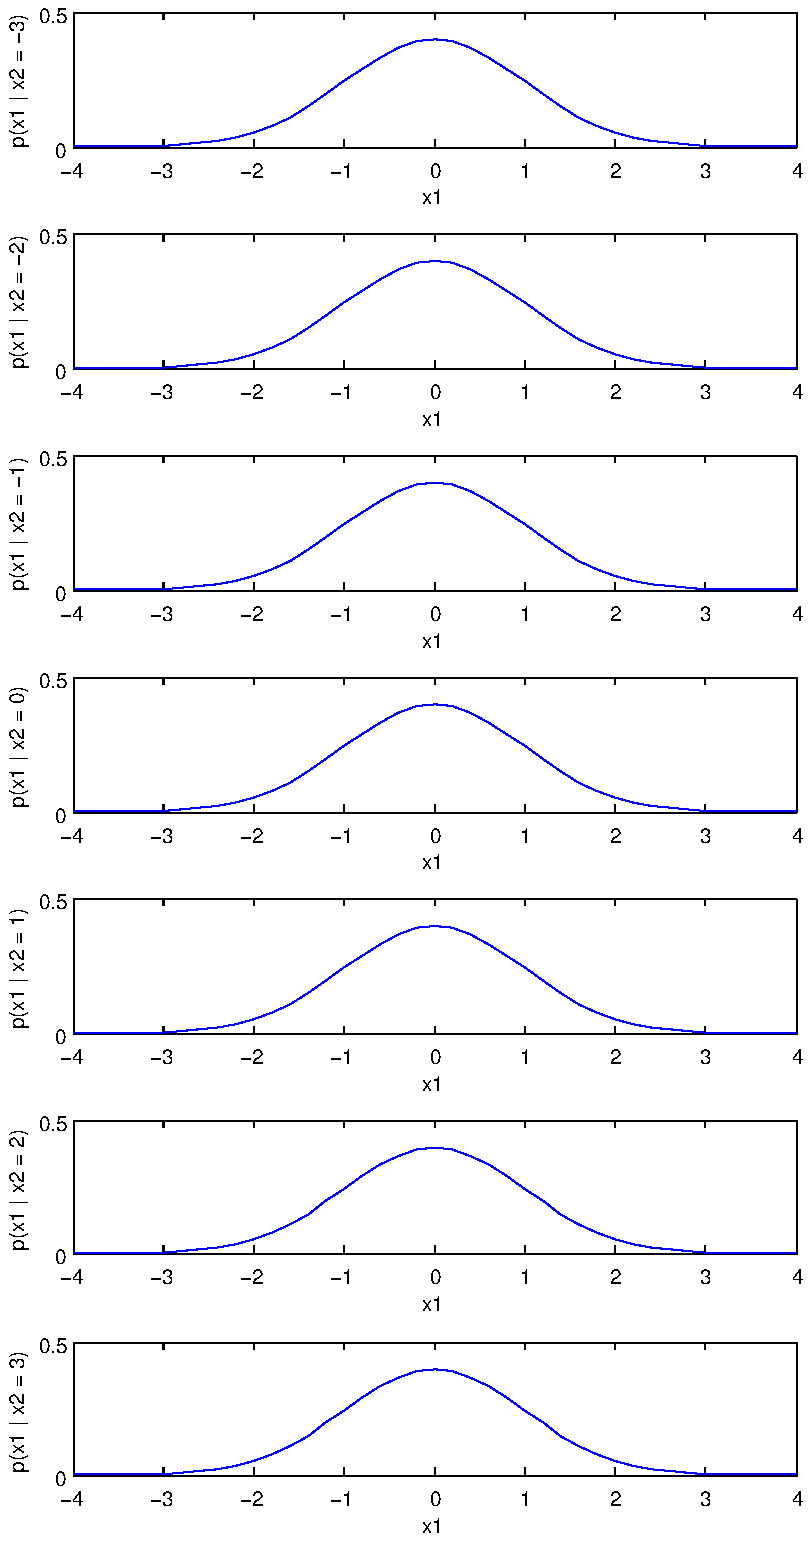
\includegraphics[width=0.8\textwidth]{ex1plot2}
  \end{center}
\end{figure}
\begin{figure}
  \begin{center}
    \caption[Surface plot of the Gaussian distribution with covariance $\cov_{1,1} = \cov_{2,2} = 1, \cov_{1,2} = \cov_{2,1} = 0.7$.]{Surface plot of the Gaussian distribution $\mathcal G_2 = \npdf(\V{x}; \mean, \cov)$ with mean $\mean = 0$ and covariance $\cov = \begin{bmatrix}1 & 0.7\\0.7 & 1\end{bmatrix}$.}
    \label{fig:plot3}
    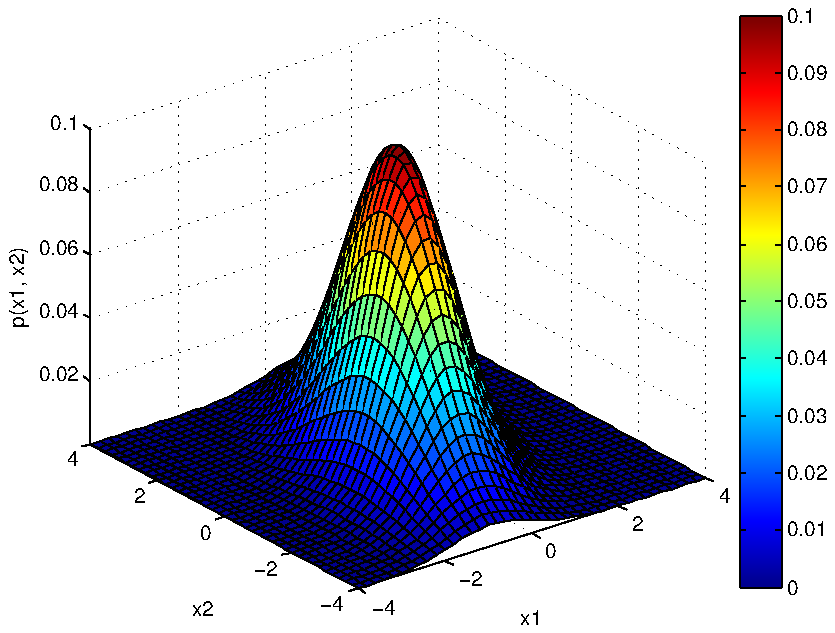
\includegraphics[width=0.8\textwidth]{ex1plot3}
  \end{center}
\end{figure}
\begin{figure}
  \begin{center}
    \caption{Plots of the conditional distribution over $x_1$ given various values for $x_2$ given the Gaussian distribution $\mathcal G_2$.  The conditional distribution over $x_1$ is plotted from top to bottom for $x_2 = -3$, $x_2 = -2$, $x_2 = -1$, $x_2 = 0$, $x_2 = 1$, $x_2 = 2$ and $x_2 = 3$.}
    \label{fig:plot4}
    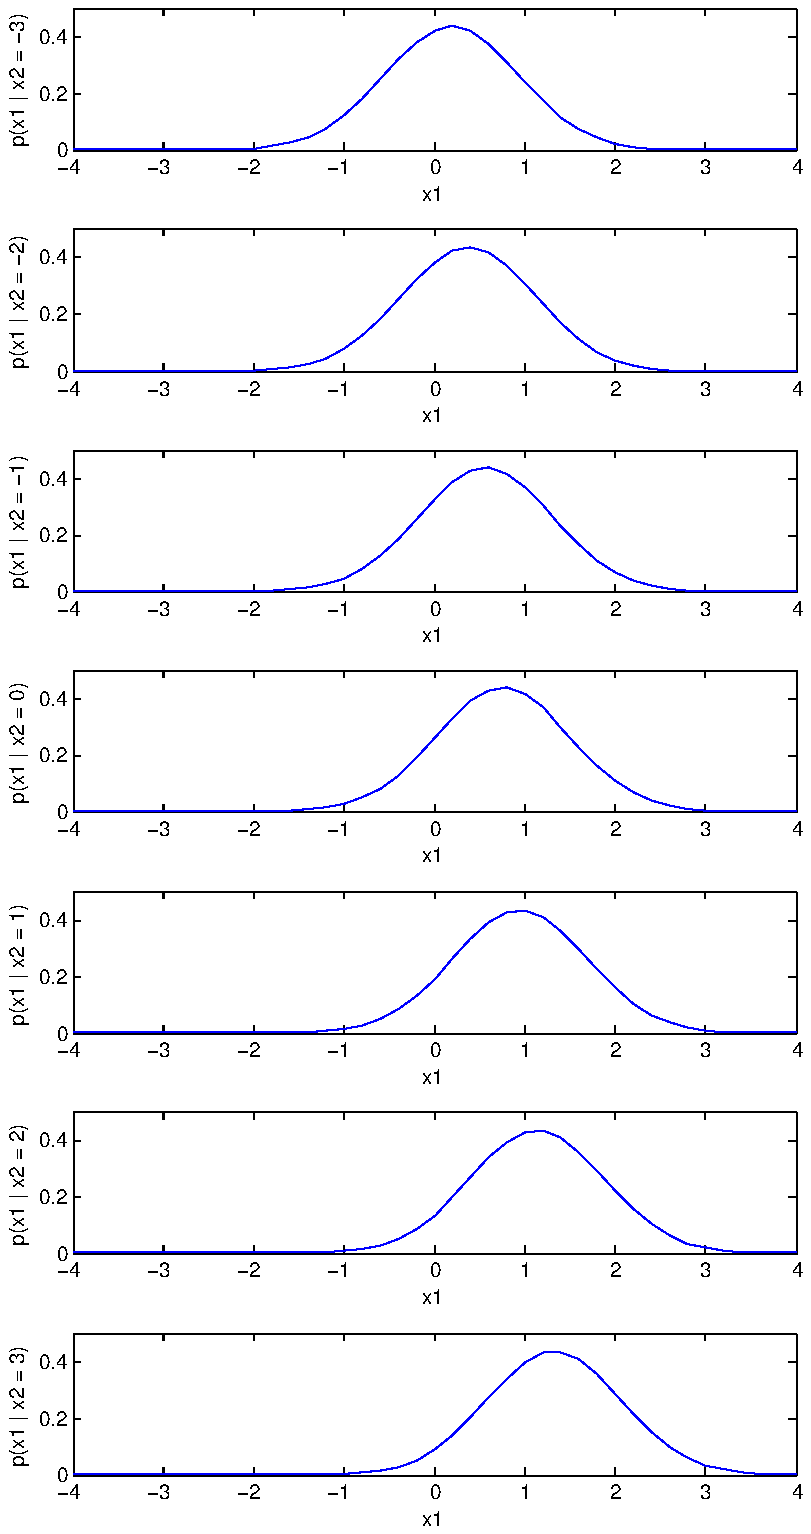
\includegraphics[width=0.8\textwidth]{ex1plot4}
  \end{center}
\end{figure}


In the first assignment, I have looked at a Gaussian distribution $\mathcal G_1 = \npdf(\V{X}; \mean, \cov)$ over two-dimensional vectors of real numbers.  The mean $\mean$ has been set to $0$, and the covariance $\cov$ to $\begin{bmatrix}1&0\\0&3\end{bmatrix}$.  The \hl{contour plot} of $\mathcal G_1$ has been plotted for input $\langle x_1, x_2 \rangle \in \V{X}$ where $-4 \leq x_1 \leq 4$ and $-4 \leq x_2 \leq 4$ in the \hl{upper part of \autoref{fig:plot1}}.  The lower part of \autoref{fig:plot1} presents the \hl{marginal distribution over }$\mhl{x_1}$.  This has been computed as $\mhl{\npdf(x_1; \mu_1, \Sigma_{1,1}) = \npdf(x_1; 0, 1)}$. 

  In \autoref{fig:plot2}, \hl{the marginal distribution} over $x_1$ for the follow values of $x_2$ are given, \hl{from top to bottom:} $\mhl{-3, -2, -1, 0, 1, 2, 3}$.  Not that these seven plots are identical to the subfigure in \autoref{fig:plot1}.  This is not really surprising, when looking at the computation:
  \begin{align*}
    p(x_1 | x_2 = v) 
    &= \npdf(x_1; \mean_1 - \Lambda_{1,1}^{-1} \Lambda_{1,2} (x_2 - \mu_2), \Lambda_{1,1}^{-1}) \\
    &= \npdf(x_1; 0 - 1  \times 0 \times v, 1) \\
    &= \npdf(x_1; 0, 1) \\
    &= p(x_1)
  \end{align*}
  with $\V{\Lambda} = \cov^{-1}$.

  Another distribution I have looked at, is $\mathcal G_2 = \npdf(\V{X}; \mean, \cov)$ with $\cov = \begin{bmatrix}1 & 0.7 \\ 0.7 & 1\end{bmatrix}$.  The \hl{surface plot is given in \autoref{fig:plot3}}.  Although the marginal distribution of $\mathcal G_1$ over $x_1$ and $\mathcal G_2$ are equal, their conditional distributions over $x_1$ given $x_2$ are not.  For $x_2 = v$, the conditional distribution is:
    \begin{align*}
      p(x_1 | x_2 = v)
      &= \npdf(x_1; \mean_1 - \Lambda_{1,1}^{-1} \Lambda_{1,2} (x_2 - \mu_2), \Lambda_{1,1}^{-1}) \\
      &= \npdf(x_1; 0 - 1.1952 \times -0.2789 \times x_2, 1.1952) \\
      &= \npdf(x_1; 0.3333 x_2, 1.1952)
    \end{align*}
\hl{The conditional distribution} over $x_1$ for $x_2 \in \left\{-3, -2, -1, 0, 1, 2, 3\right\}$ is presented in \hl{\autoref{fig:plot4}}.


\section{Gaussian Processes}
In this exercise, the temperature must be predicted from the number of chirps per time unit crickets produce during summer.  The dataset describing the data to learn from, \texttt{chirps.mat}, contains only 15 chirp-temperature pairs.  Because of this small dataset size, the \hl{test set contains 1 data point}, and \hl{14-fold cross-validation} is applied to acquire the best learner.  A plot of the dataset is given in \autoref{fig:ex2plot1}.


\begin{figure}
  \begin{center}
  \caption{A plot of the dataset \texttt{chirps.mat}.  The red ``$\color{red}+$'''s represent the train data points. The blue ``$\color{blue}\times$''' represent the test data point.}
    \label{fig:ex2plot1}
    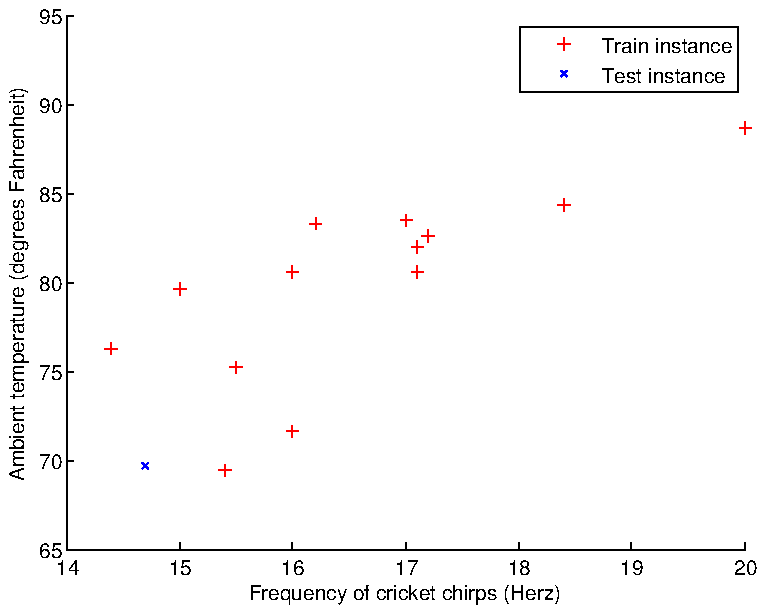
\includegraphics[width=0.8\textwidth]{ex2plot1}
  \end{center}
\end{figure}


I have written an implementation of Gaussian process according to Algorithm 1 from the assignment in MATLAB in \texttt{gaussian\_process.m}.  The implementation has been done as close as possible to the pseudocode.  The \texttt{gaussian\_process} function has the following inputs:
\begin{itemize}
\item $\T{X}$: an $\T{N}$ by $\T{D}$ matrix, representing $\T{N}$ data points of dimensionality $\T{D}$, which are used for training.
\item $\T{t}$: an $\T{N}$ by $\T{1}$ vector.  These are the target values, which the Gaussian process should approximate.
\item $\T{k}$: the kernel function.  This function should accept two arguments, both $\T{1}$ by $\T{D}$ dimensional vectors.
\item $\T{sigma2}$: the squared variance on the target value.  This represents the amount of noise in the data.
\item $\T{x\_}$: a data point, for which the Gaussian process shall predict the target value.
\end{itemize}
As in the pseudocode, the provided MATLAB implementation returns three values:
\begin{itemize}
\item $\T{f\_}$: the most likely target value, given the input properties.
\item $\T{sigma\_2}$: the squared variance on the prediction.
\item $\T{LLog}$: the log-likelihood of the provided train data under the model.  This can also be seen as a measure how well the model can ``explain'' the data.
\end{itemize}  

The exercise tells that $\T{sigma2}$ should have a small value.  Therefore it is set to $10^{-7}$, unless stated differently.

The kernel function $k(\V{x}, \V{x}')$ as defined by Equation 9 is returned by calling \texttt{squared\_exponential} with specific values for $\theta$ and $l$, called the hyperparameters.  These parameters represent a quantity associated with the spread of the temperature and chirp frequency in the train data set.

Learning from data in terms of Gaussian processes means to find the Gaussian process under which the dataset is most likely to occur.  This means that the program needs to find values for the hyperparameters of the kernel function $k$ which \hl{maximize the (log-)likelihood}.  In this case, the software has to optimize the log-likelihood by finding the correct values of $\theta$ and $l$.  This can be done in two ways:
\begin{itemize}
\item Gradient ascent.  For this, I need to compute the gradient with respect to $\theta$ and $l$ of the following expression:
\begin{align*}
- \frac{1}{2}\V{t}^\top (\V{K} \backslash \V{t}) - \sum_i \log \chol(\V{K}) - \frac{N}{2} \log 2\pi
\end{align*}
where $\V{t}$ are the labels of the train data, $N$ the size of the train data set, and $\V{K}$ a matrix with values $K_{ij} = k(x_i, x_j)$ for elements $x_i, x_j$ in the dataset $\V{X}$.

Although this will give the best result, finding the gradient of this expression is very hard.

\item Grid search.  With a grid search, I will look for the highest log-likelihood of the Gaussian process for values of $\theta$ and $l$ in a certain range and step size.

When applying this method, the best combination of the hyperparameters might not be found, because that optimum might be in between two steps, or outside the searching range.
\end{itemize}
I have also searched for the hyperparameters which minimize the estimated error, as well as maximize the variance.

The \hl{estimated error} of the Gaussian process will be measured by the \hl{mean square error} of the predicted mean temperature, associated with the input chirp frequency.  For $n$ targets $\V{t}$ and their corresponding predictions $\V{t}^\ast$, the error is given by:
\begin{align*}
\err(\V{t}, \V{t}^\ast)
  &= \frac{1}{n} \sum_i^n \left(t_i - t^\ast_i\right)^2
\end{align*}
A performance measure should increase when the inspected subject behaves (in this case, generalizes) more to our likings.  Therefore, I will define the \hl{performance measure} as the \hl{negative of the estimated error}.

I have decided to apply the \hl{grid search approach}.  The lower and upper bounds on the search range have been based on the data in terms of the average temperature and chirps among the data points.  Let $\bar\theta$ and $\bar l$ be the average temperature and average chirp frequency among the test-and-validation set.  For ease of reading, I will use $\V{\bar\theta} = \begin{bmatrix}\bar\theta\\\bar l\end{bmatrix}$ and $\V{\theta} = \begin{bmatrix}\theta\\l\end{bmatrix}$ as shorthands.  Initially, I have looked at the joined ranges $[0.1\V{\bar\theta}, \V{\bar\theta}]$ with step size $\dif \V{\theta} = 0.1\V{\bar\theta}$, and $(\V{\bar\theta}, 100 \V{\bar\theta}]$ with step size $\dif \V{\theta} = \V{\bar\theta}$\footnote{At first, I wanted to look at the range $[0.1\V{\bar\theta}, 100\V{\bar\theta}]$ with step size $0.1\V{\bar\theta}$. Combining this with the cross validation, I would test 14 million Gaussian processes.  After I have implemented the cross-validation part in a multithreading way and ran it overnight on a quadcore pc with no other big tasks, and the algorithm had not finished in the afternoon, I came to the conclusion this must not have been the idea.}.  %The log-likelihood, error and squared variance have been plotted against the values of $\theta$ and $l$ in the aforementioned ranges in \autoref{fig:ex2plot2log}, \autoref{fig:ex2plot2err} and \autoref{fig:ex2plot2var}.

The results of the grid search, for noise levels $\sigma^2 = 10^{-7}$ and $\sigma^2 = 10^{-4}$, and tests sets of 1 up to 5 items, are presented in \autoref{tab:s7} and \autoref{tab:s4}.  In the first column, the noise level is indicated.  The second column contains data on how many test items have been used.  In the third and fourth column can be found which heuristic has been optimized, and what its optimal value is.  Optimization has been done as described above; log-likelihood and variance are maximized, while the expected error is minimized.  In the sixth and seventh column are recorded the optimal values $\V{\hat\theta}$ for the heuristic.  The last column presents the performance.

In \hl{\autoref{fig:ex2plot3}}, one can find the \hl{expected mean and its variance for input values 12 through 22} for various values of $\V{\hat\theta}$.  The expected mean and variance for the parameterization which optimizes the log-likelihood is drawn as a red line.  The expected mean and variance generated by $\V{\hat\theta}$ for a minimal error is supplied in green.  The blue line is generated by $\V{\hat\theta}$ which maximize the variance.  The corresponding values for $\V{\hat\theta} = \begin{bmatrix}\hat\theta \\\hat l\end{bmatrix}$ can be found in \autoref{tab:s7}.

It is notable that, although the \hl{variance} is so low that it cannot be distinguished from the mean for most part of the lines in \autoref{fig:ex2plot3}, it (even visually) \hl{increases for inputs which are further} from train data points.  This is not surprising; the further you are from known data, the less precise your estimation will be.  Because variance is a measure of confidence, this is only expected.

\begin{table}
  \caption{The performance of Gaussian processes based on differently selected hyperparameters $\hat\theta$ and $\hat l$ with noise level $\sigma^2=10^{-7}$.}
  \label{tab:s7}
  \begin{tabular}{cclcccc}
    \hline
    $\sigma^2$ & Test items & Criterion & Cr.\ value & $\hat\theta$ & $\hat l$ & Performance \\
    \hline
    \hline
    $10^{-7}$ & 1 & Log-likelihood & $-1.777 \times 10^8$ & $0.2\bar\theta$ & $93 \bar l$ & $-75.422834$ \\
              &   & Expected error & $3.067816$ & $0.7\bar\theta$ & $\bar l$ & $-112.484638$ \\
              &   & Variance & $1.050682$ & $0.1\bar\theta$ & $98\bar l$ & $-75.563232$ \\
    \hline
              & 2 & Log-likelihood & $-1.777 \times 10^8$ & $0.2\bar\theta$ & $93 \bar l$ & $-79.125398$ \\
              &   & Expected error & $3.067816$ & $0.7\bar\theta$ & $\bar l$ & $-100.501221$ \\
              &   & Variance & $1.050682$ & $0.1\bar\theta$ & $98\bar l$ & $-79.062857$ \\
    \hline
              & 3 & Log-likelihood & $-1.777 \times 10^8$ & $0.2\bar\theta$ & $93 \bar l$ & $-78.9199$ \\
              &   & Expected error & $3.067816$ & $0.7\bar\theta$ & $\bar l$ & $-90.315318$ \\
              &   & Variance & $1.050682$ & $0.1\bar\theta$ & $98\bar l$ & $-78.967861$ \\
    \hline
              & 4 & Log-likelihood & $-1.777 \times 10^8$ & $0.2\bar\theta$ & $93 \bar l$ & $-79.130449$ \\
              &   & Expected error & $3.067816$ & $0.7\bar\theta$ & $\bar l$ & $-98.082120$ \\
              &   & Variance & $1.050682$ & $0.1\bar\theta$ & $98\bar l$ & $-78.554024$ \\
    \hline
              & 5 & Log-likelihood & $-1.777 \times 10^8$ & $0.2\bar\theta$ & $93 \bar l$ & $-70.188813$ \\
              &   & Expected error & $3.067816$ & $0.7\bar\theta$ & $\bar l$ & $-69.918030$ \\
              &   & Variance & $1.050682$ & $0.1\bar\theta$ & $98\bar l$ & $-71.878425$ \\
    \hline
  \end{tabular}
\end{table}
\begin{table}
  \caption{The performance of Gaussian processes based on differently selected hyperparameters $\hat\theta$ and $\hat l$ with noise level $\sigma^2=10^{-4}$.}
  \label{tab:s4}
  \begin{tabular}{cclcccc}
    \hline
    $\sigma^2$ & Test items & Criterion & Cr.\ value & $\hat\theta$ & $\hat l$ & Performance \\
    \hline
    \hline
    $10^{-4}$ & 1 & Log-likelihood & $-177937.199801$ & $0.4\bar\theta$ & $98 \bar l$ & $-75.7453$ \\
              &   & Expected error & $3.043957$ & $0.8\bar\theta$ & $1.1\bar l$ & $-84.724637$ \\
              &   & Variance & $1.050777$ & $0.1\bar\theta$ & $98\bar l$ & $-75.6286$ \\
    \hline
              & 2 & Log-likelihood & $-175634.144192$ & $0.3\bar\theta$ & $98 \bar l$ & $-78.6657$ \\
              &   & Expected error & $7.861724$ & $0.1\bar\theta$ & $\bar l$ & $-84.7246$ \\
              &   & Variance & $0.000088$ & $0.1\bar\theta$ & $98\bar l$ & $-75.6286$ \\
    \hline
              & 3 & Log-likelihood & $-4215.151426$ & $0.4\bar\theta$ & $98 \bar l$ & $-78.953028$ \\
              &   & Expected error & $8.514720$ & $0.9\bar\theta$ & $0.1\bar l$ & $-82342356$ \\
              &   & Variance & $25.881656$ & $0.1\bar\theta$ & $98\bar l$ & $-78.965517$ \\
    \hline
              & 4 & Log-likelihood & $-4123.566594$ & $0.3\bar\theta$ & $98 \bar l$ & $-77.410747$ \\
              &   & Expected error & $0.621619$ & $2\bar\theta$ & $85\bar l$ & $-77.931735$ \\
              &   & Variance & $11.443740$ & $0.1\bar\theta$ & $98\bar l$ & $-77.452683$ \\
    \hline
              & 5 & Log-likelihood & $-4037.452951$ & $0.3\bar\theta$ & $98 \bar l$ & $-77.516761$ \\
              &   & Expected error & $1.525246$ & $0.6\bar\theta$ & $1.2 \bar l$ & $-69.502743$ \\
              &   & Variance & $13.491900$ & $0.1\bar\theta$ & $98\bar l$ & $-77.912734$ \\
    \hline
  \end{tabular}
\end{table}
%\begin{table}
%  \caption{The performance of Gaussian processes based on differently selected hyperparameters $\hat\theta$ and $\hat l$ with noise level $\sigma^2=10^{-1}$.}
%  \label{tab:s1}
%  \begin{tabular}{cclcccc}
%    \hline
%    $\sigma^2$ & Test items & Criterion & Cr.\ value & $\hat\theta$ & $\hat l$ & Performance \\
%    \hline
%    \hline
%    $10^{-4}$ & 1 & Log-likelihood & $-4037.452951$ & $0.3\bar\theta$ & $98 \bar l$ & $-$ \\
%              &   & Expected error & $1.525246$ & $0.6\bar\theta$ & $1.2\bar l$ & $-$ \\
%              &   & Variance & $13.491900$ & $0.1\bar\theta$ & $98\bar l$ & $-$ \\
%    \hline
%              & 2 & Log-likelihood & $-4037.452951$ & $0.3\bar\theta$ & $98 \bar l$ & $-$ \\
%              &   & Expected error & $1.525246$ & $0.6\bar\theta$ & $1.2\bar l$ & $-$ \\
%              &   & Variance & $13.491900$ & $0.1\bar\theta$ & $98\bar l$ & $-$ \\
%    \hline
%              & 3 & Log-likelihood & $-4037.452951$ & $0.3\bar\theta$ & $98 \bar l$ & $-$ \\
%              &   & Expected error & $1.525246$ & $0.6\bar\theta$ & $1.2\bar l$ & $-$ \\
%              &   & Variance & $13.491900$ & $0.1\bar\theta$ & $98\bar l$ & $-$ \\
%    \hline
%              & 4 & Log-likelihood & $-4037.452951$ & $0.3\bar\theta$ & $98 \bar l$ & $-$ \\
%              &   & Expected error & $1.525246$ & $0.6\bar\theta$ & $1.2\bar l$ & $-$ \\
%              &   & Variance & $13.491900$ & $0.1\bar\theta$ & $98\bar l$ & $-$ \\
%    \hline
%              & 5 & Log-likelihood & $-4037.452951$ & $0.3\bar\theta$ & $98 \bar l$ & $-$ \\
%              &   & Expected error & $1.525246$ & $0.6\bar\theta$ & $1.2 \bar l$ & $-$ \\
%              &   & Variance & $13.491900$ & $0.1\bar\theta$ & $98\bar l$ & $-$ \\
%    \hline
%  \end{tabular}
%\end{table}

%\begin{figure}
%  \begin{center}
%    \caption{The log-likelihood returned by the Gaussian process has been plotted against hyperparameters $\theta, l$.  Both hyperparameters are in the range of a tenth of its average in the dataset up to hundred times the average.  Higher, red values for the log-likelihood are more desirable.}
%    \label{fig:ex2plot2log}
%  \end{center}
%\end{figure}
%\begin{figure}
%  \begin{center}
%    \caption{The error of the Gaussian process has been plotted against hyperparameters $\theta, l$.  Both hyperparameters are in the range of a tenth of its average in the dataset up to hundred times the average.  The error is measured as the mean square error among the test samples.  Lower, blue values for the mean square error are more desirable.}
%    \label{fig:ex2plot2err}
%  \end{center}
%\end{figure}
%\begin{figure}
%  \begin{center}
%    \caption{The squared variance of the Gaussian process has been plotted against hyperparameters $\theta, l$.  Both hyperparameters are in the range of a tenth of its average in the dataset up to hundred times the average.  The error is measured as the mean square error among the test samples.}
%    \label{fig:ex2plot2var}
%  \end{center}
%\end{figure}

\begin{figure}
  \begin{center}
    \caption{The expected means together with the variance generated by the Gaussian process, with $\sigma^2=10^{-7}$ and 14 train data points.  The red line represents the means generated with the hyperparameters which optimize the log-likelihood $\hat\theta = 0.2\bar\theta$, $\hat l = 93\bar l$.  The blue line is parameterized with $\hat\theta=0.7\bar\theta, \hat l = \bar l$, which minimize the expected mean square error.  The green line is generated with $\hat\theta=0.1\bar\theta, \hat l = 98\bar l$.  The variance is on most places not visible, as it is really close to the mean.}
    \label{fig:ex2plot3}
    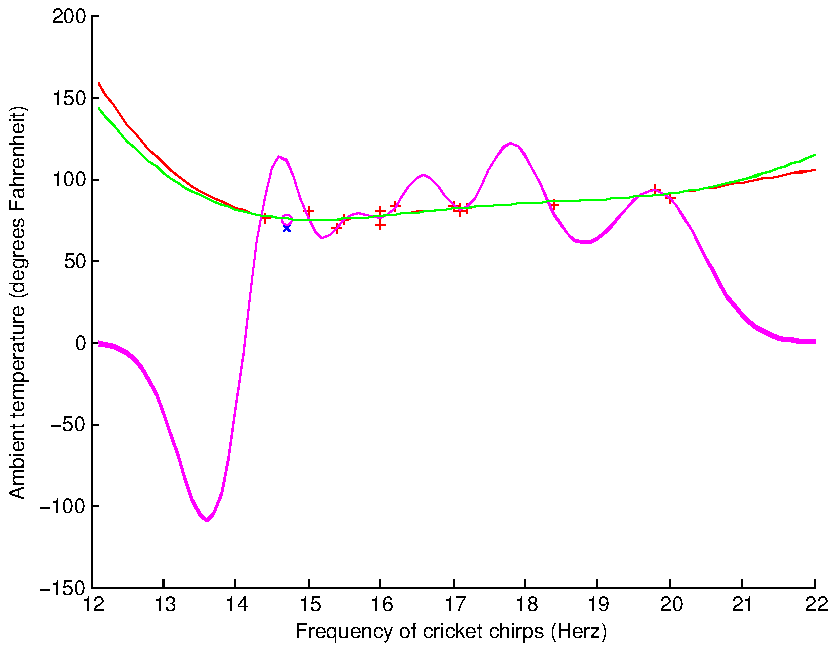
\includegraphics[width=0.8\textwidth]{ex2plot3}
  \end{center}
\end{figure}
\end{document}
